\subsection{About MATLAB}
\begin{frame}{About MATLAB}
\begin{itemize}
\item Commercial and experience (<-> Octave)
\item Not for general purpose (no one will write an operating system using MATLAB)
\item Excel at numerical calculations and plot
\item Many useful toolboxes (though we will not cover these in this course, you will use some of them in advanced courses)
\item Widely used in academia
\end{itemize}
\end{frame}

\subsection{Interface}
\begin{frame}{Interface}
\begin{figure}[htbp]
\centering
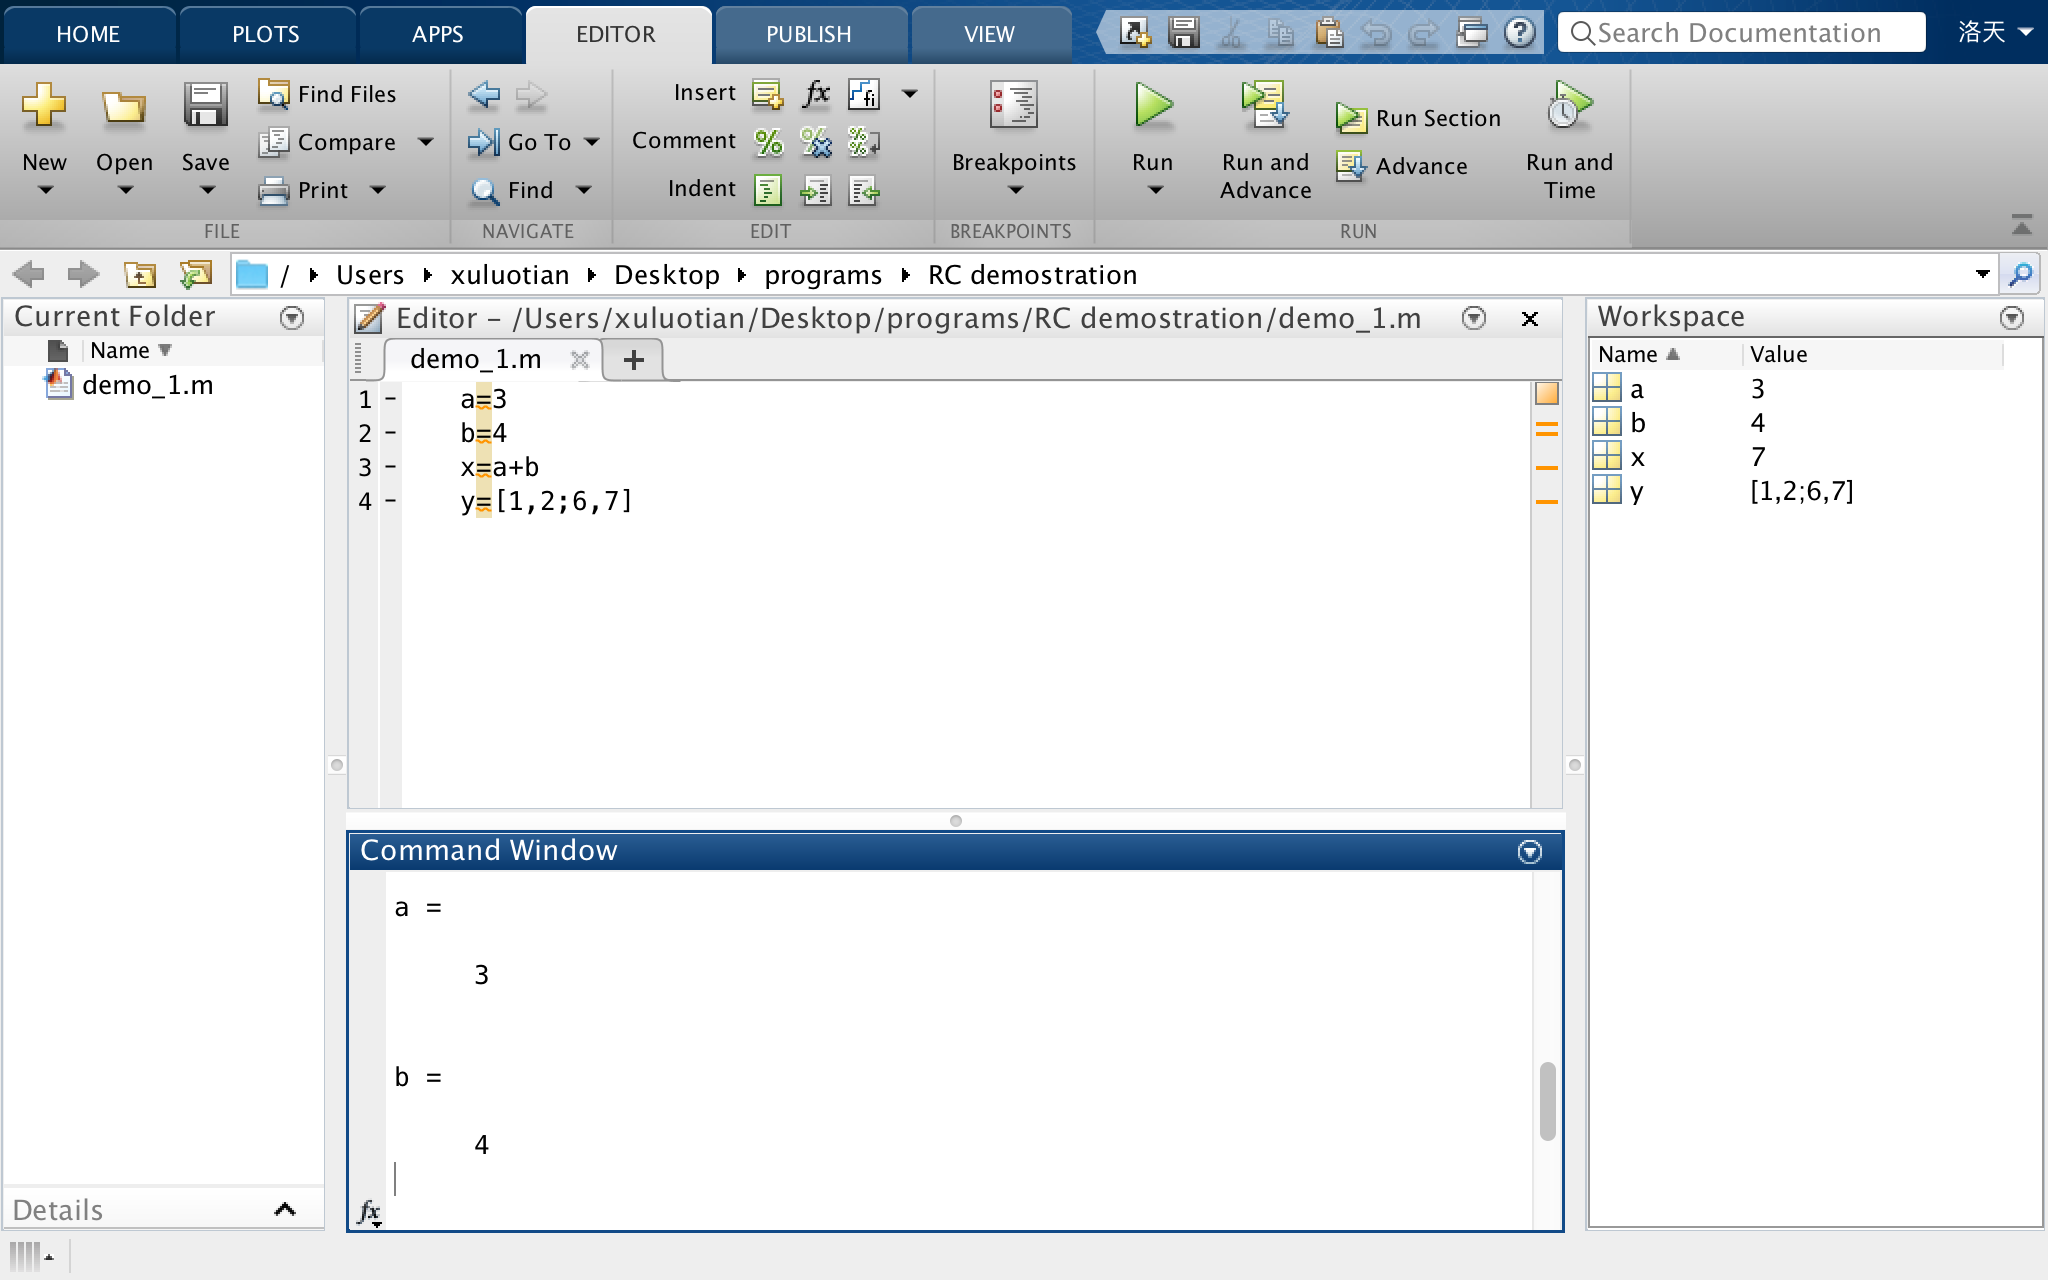
\includegraphics[width=0.95\textwidth]{pic/window.png}
\end{figure}
\end{frame}

\begin{frame}{Interface}
\begin{block}{Workspace}
Store and show what variables are available and their value. You can double-click a variable to see its details (useful for matrix). You can also save and load workspace.
\end{block}
\begin{block}{Command Window}
Input command direct into the command line. Variables can be seen in the workspace.
\end{block}
\begin{block}{Editor}
Editor is actually where you ``buffer'' your commands. \textbf{Run} the code in the editor is equivalent to type the command line by line into command window.
\end{block}
\end{frame}


\begin{frame}{Interface}
\begin{block}{Current Folder (\& Environment)}
It indicates which folder you are currently. When you operate on file (e.g. call a function from another file), MATLAB will search the file in current directory or search path. Personally, I suggest managing your file in the current directory, which will make your life easier.

For more details about search path, you can refer to \url{https://ww2.mathworks.cn/help/matlab/matlab_env/what-is-the-matlab-search-path.html?lang=en}.
\end{block}
\end{frame}

\subsection{Syntax}
\begin{frame}{Operators \& Keys}
\begin{itemize}
\item ``+'', ``-'', ``*'', ``/'', ``.*'', ``./'', ``\ \^\ '', ``\ .\^\ '': matrix or elementwise arithmetic
\item ``='': assignment
\item ``=='': equal
\item ``\&\&'', ``||'': logicial and / or
\item ``\%'': comment. Will be ignored by MATLAB. Make the code easier to understand
\item ``;'': suppress output. Please add it to every line that you do not expect output! Extra output may result in dection
\item ``$\uparrow$, $\downarrow$'': view history
\item Tab: indent
\item ``clc'': clear command window
\item ``clear / clear all'': clear workspace
\end{itemize}
\end{frame}

\begin{frame}{Some Special Variables \& Constants}
\begin{block}{Tips}
\textbf{All variables in MATLAB are matrix.} Scalar is essential a $1\times1$ matix, but it allows some operations that may be invalid for a $1\times1$ matrix.
\end{block}
\begin{itemize}
\item ``ans'': default output variable; do not use ``ans'' as your own variable name in your script
\item ``i'', ``j'': virtual number
\item ``Inf'': infinite
\item ``NaN'': not a number; mostly appear when the result exceed some limit or some errors occur
\item ``pi''
\end{itemize}

\begin{block}{save \& load}
\begin{itemize}
\item save xxx: save all current variables into .mat file
\item load xxx: load .mat file; will not clear variables alread in workspace; will cover the variable in workspace if two variables share same name
\end{itemize}
\end{block}
\end{frame}

\begin{frame}{Command}
\begin{itemize}
\item ``exist'': test the existence of a varibale or a file (exist xxx)
\item ``global'': declare global variable
\item ``help'', ``doc'': show document (help xxx; doc xxx)
\item ``clc'': clear command window
\item ``clear / clear all'': clear workspace
\end{itemize}
It's good habit to add ``clc'' and ``clear'' at the first of your program, \textbf{especially in your homework}.
\end{frame}

\begin{frame}{Control Flow}
\begin{itemize}
\item if, while, for
\item while 1
\end{itemize}
\begin{minipage}{0.05\textwidth}
~\\
\end{minipage}
\begin{minipage}{0.5\textwidth}
\lstinputlisting[language=Matlab]{code/control_flow_demo.m}
\end{minipage}
\begin{minipage}{0.05\textwidth}
~\\
\end{minipage}
\begin{minipage}{0.35\textwidth}
Outputs: \\
1 $\hookleftarrow$ \\
2 $\hookleftarrow$ \\
3 $\hookleftarrow$ \\
4 $\hookleftarrow$ \\
look, it is a four! $\hookleftarrow$ \\
5 $\hookleftarrow$ \\
100 $\hookleftarrow$ \\
99 $\hookleftarrow$ \\
98 $\hookleftarrow$ \\
97 $\hookleftarrow$ \\
96 $\hookleftarrow$ \\
\end{minipage}
\end{frame}

\begin{frame}{Control Flow}
\begin{itemize}
\item break: break the loop
\item continue: ignore the later code in this iteration; skip directly to the next iteration
\end{itemize}
\begin{minipage}{0.05\textwidth}
~\\
\end{minipage}
\begin{minipage}{0.5\textwidth}
\lstinputlisting[language=Matlab]{code/break_cont_demo.m}
\end{minipage}
\begin{minipage}{0.05\textwidth}
~\\
\end{minipage}
\begin{minipage}{0.35\textwidth}
Outputs: \\
9 $\hookleftarrow$ \\
6 $\hookleftarrow$ \\
5 $\hookleftarrow$ \\
4 $\hookleftarrow$ \\
3 $\hookleftarrow$ \\
\end{minipage}
\end{frame}

\begin{frame}{M-file}
Source code of MATLAB code is stored in .m files. It is essential text file, which means actually you can modify it as for .txt file. There are two kinds of .m file: script and function.
\begin{block}{script}
Scripts are essentially putting the code line by line to the command window. A script has no specific input and output. It operates on the value of workspace. Note that, if you do not clear the workspace before running a scipt, all variables in the workspace will be used by script, so of which are not intended, and may cause what you call ``XUANXUE'' (dark magic). \footnotemark
\end{block}
\begin{block}{function}
Functions take specific input and produce output. A function only working on its own varivales, which you can take it as a separate box. It promotes \textbf{code reuse} and \textbf{decoupling}.
\end{block}
\footnotetext{So you see why I mention adding ``clear'' in the front of your code is a good habit.}
\end{frame}

\begin{frame}{M-file}

\begin{block}{Aside: Code Reuse \& Decoupling\footnotemark\footnotemark}
Code reuse not only means less code you need to produce; more importantly, it means less code you need to take care (debug, modify, or performance improvement). Decoupling means we would like the code be separated into modules, and limit the coupling only to the interfaces, i.e. where modules connect.
\end{block}
\begin{minipage}{0.48\textwidth}
	\structure{Low coupling:}
	\begin{figure}
		\centering
		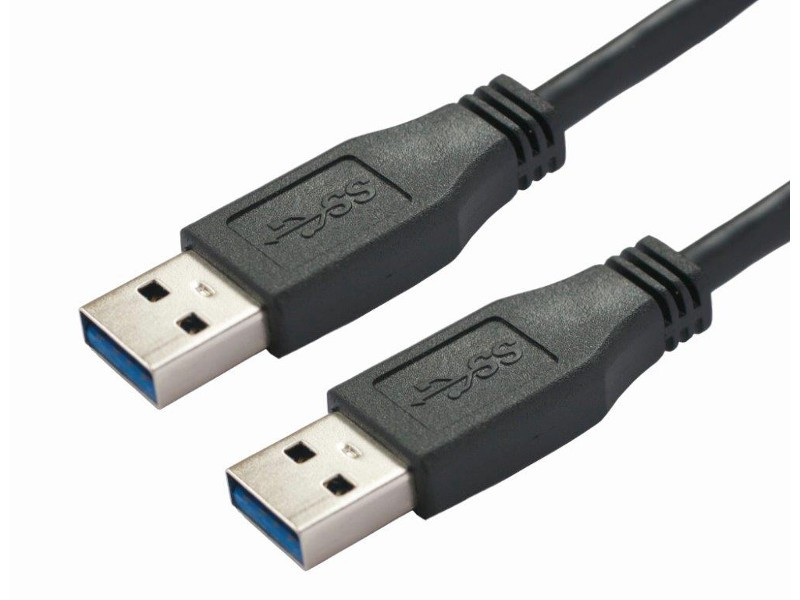
\includegraphics[width=0.4\textwidth]{pic/low-coupling.jpg}
	\end{figure}
\end{minipage}
\begin{minipage}{0.48\textwidth}
	\structure{High coupling:}
	\begin{figure}
		\centering
		
\includegraphics[width=0.4\textwidth]{pic/high-coupling.jpg}
	\end{figure}
\end{minipage}
\footnotetext[2]{``Aside'' means the content below will be discussed in more advanced courses, but it can be quite helpful if you know it now.}
\footnotetext[3]{Reference and thanks: some of content is from \url{https://github.com/tripack45/VE280-Notes}.}
\end{frame}